%%%% ijcai26.tex

\typeout{IJCAI--ECAI 26 Instructions for Authors}

\documentclass{article}
\pdfpagewidth=8.5in
\pdfpageheight=11in

\usepackage{ijcai26}

\usepackage{times}
\usepackage{soul}
\usepackage{url}
\usepackage[hidelinks]{hyperref}
\usepackage[utf8]{inputenc}
\usepackage[small]{caption}
\usepackage{graphicx}
\usepackage{amsmath}
\usepackage{amsthm}
\usepackage{booktabs}
\usepackage{algorithm}
\usepackage{algorithmic}
\usepackage[switch]{lineno}
\usepackage{xcolor}
\usepackage{tabularx}
\usepackage{makecell}
\usepackage{multirow}
\usepackage{tabularx}

\usepackage{float}
\usepackage{afterpage}


% Comment out this line in the camera-ready submission
\linenumbers

\urlstyle{same}

\newtheorem{example}{Example}
\newtheorem{theorem}{Theorem}

\pdfinfo{
/TemplateVersion (IJCAI.2026.0)
}

\title{Evaluating Demographic Misrepresentation in Image-to-Image Portrait Editing}

% Single author syntax (replace for submission as appropriate)
\author{
    Anonymous Submission
    \affiliations
    \emails
}
% Multiple author syntax (optional)
\iffalse
\author{
First Author$^1$
\and
Second Author$^2$\and
Third Author$^{2,3}$\And
Fourth Author$^4$\\
\affiliations
$^1$First Affiliation\\
$^2$Second Affiliation\\
$^3$Third Affiliation\\
$^4$Fourth Affiliation\\
\emails
\{first, second\}@example.com,
third@other.example.com,
fourth@example.com
}
\fi

\begin{document}

\makeatletter
% Redefine maketitle to include figure
\renewcommand{\maketitle}{%
 \par
 \begingroup
   \def\thefootnote{\fnsymbol{footnote}}
   \def\@makefnmark{$^{\@thefnmark}$}
   \twocolumn[{\@maketitle
   \begin{center}
       \vspace{-1.5cm}
       \centering \small
       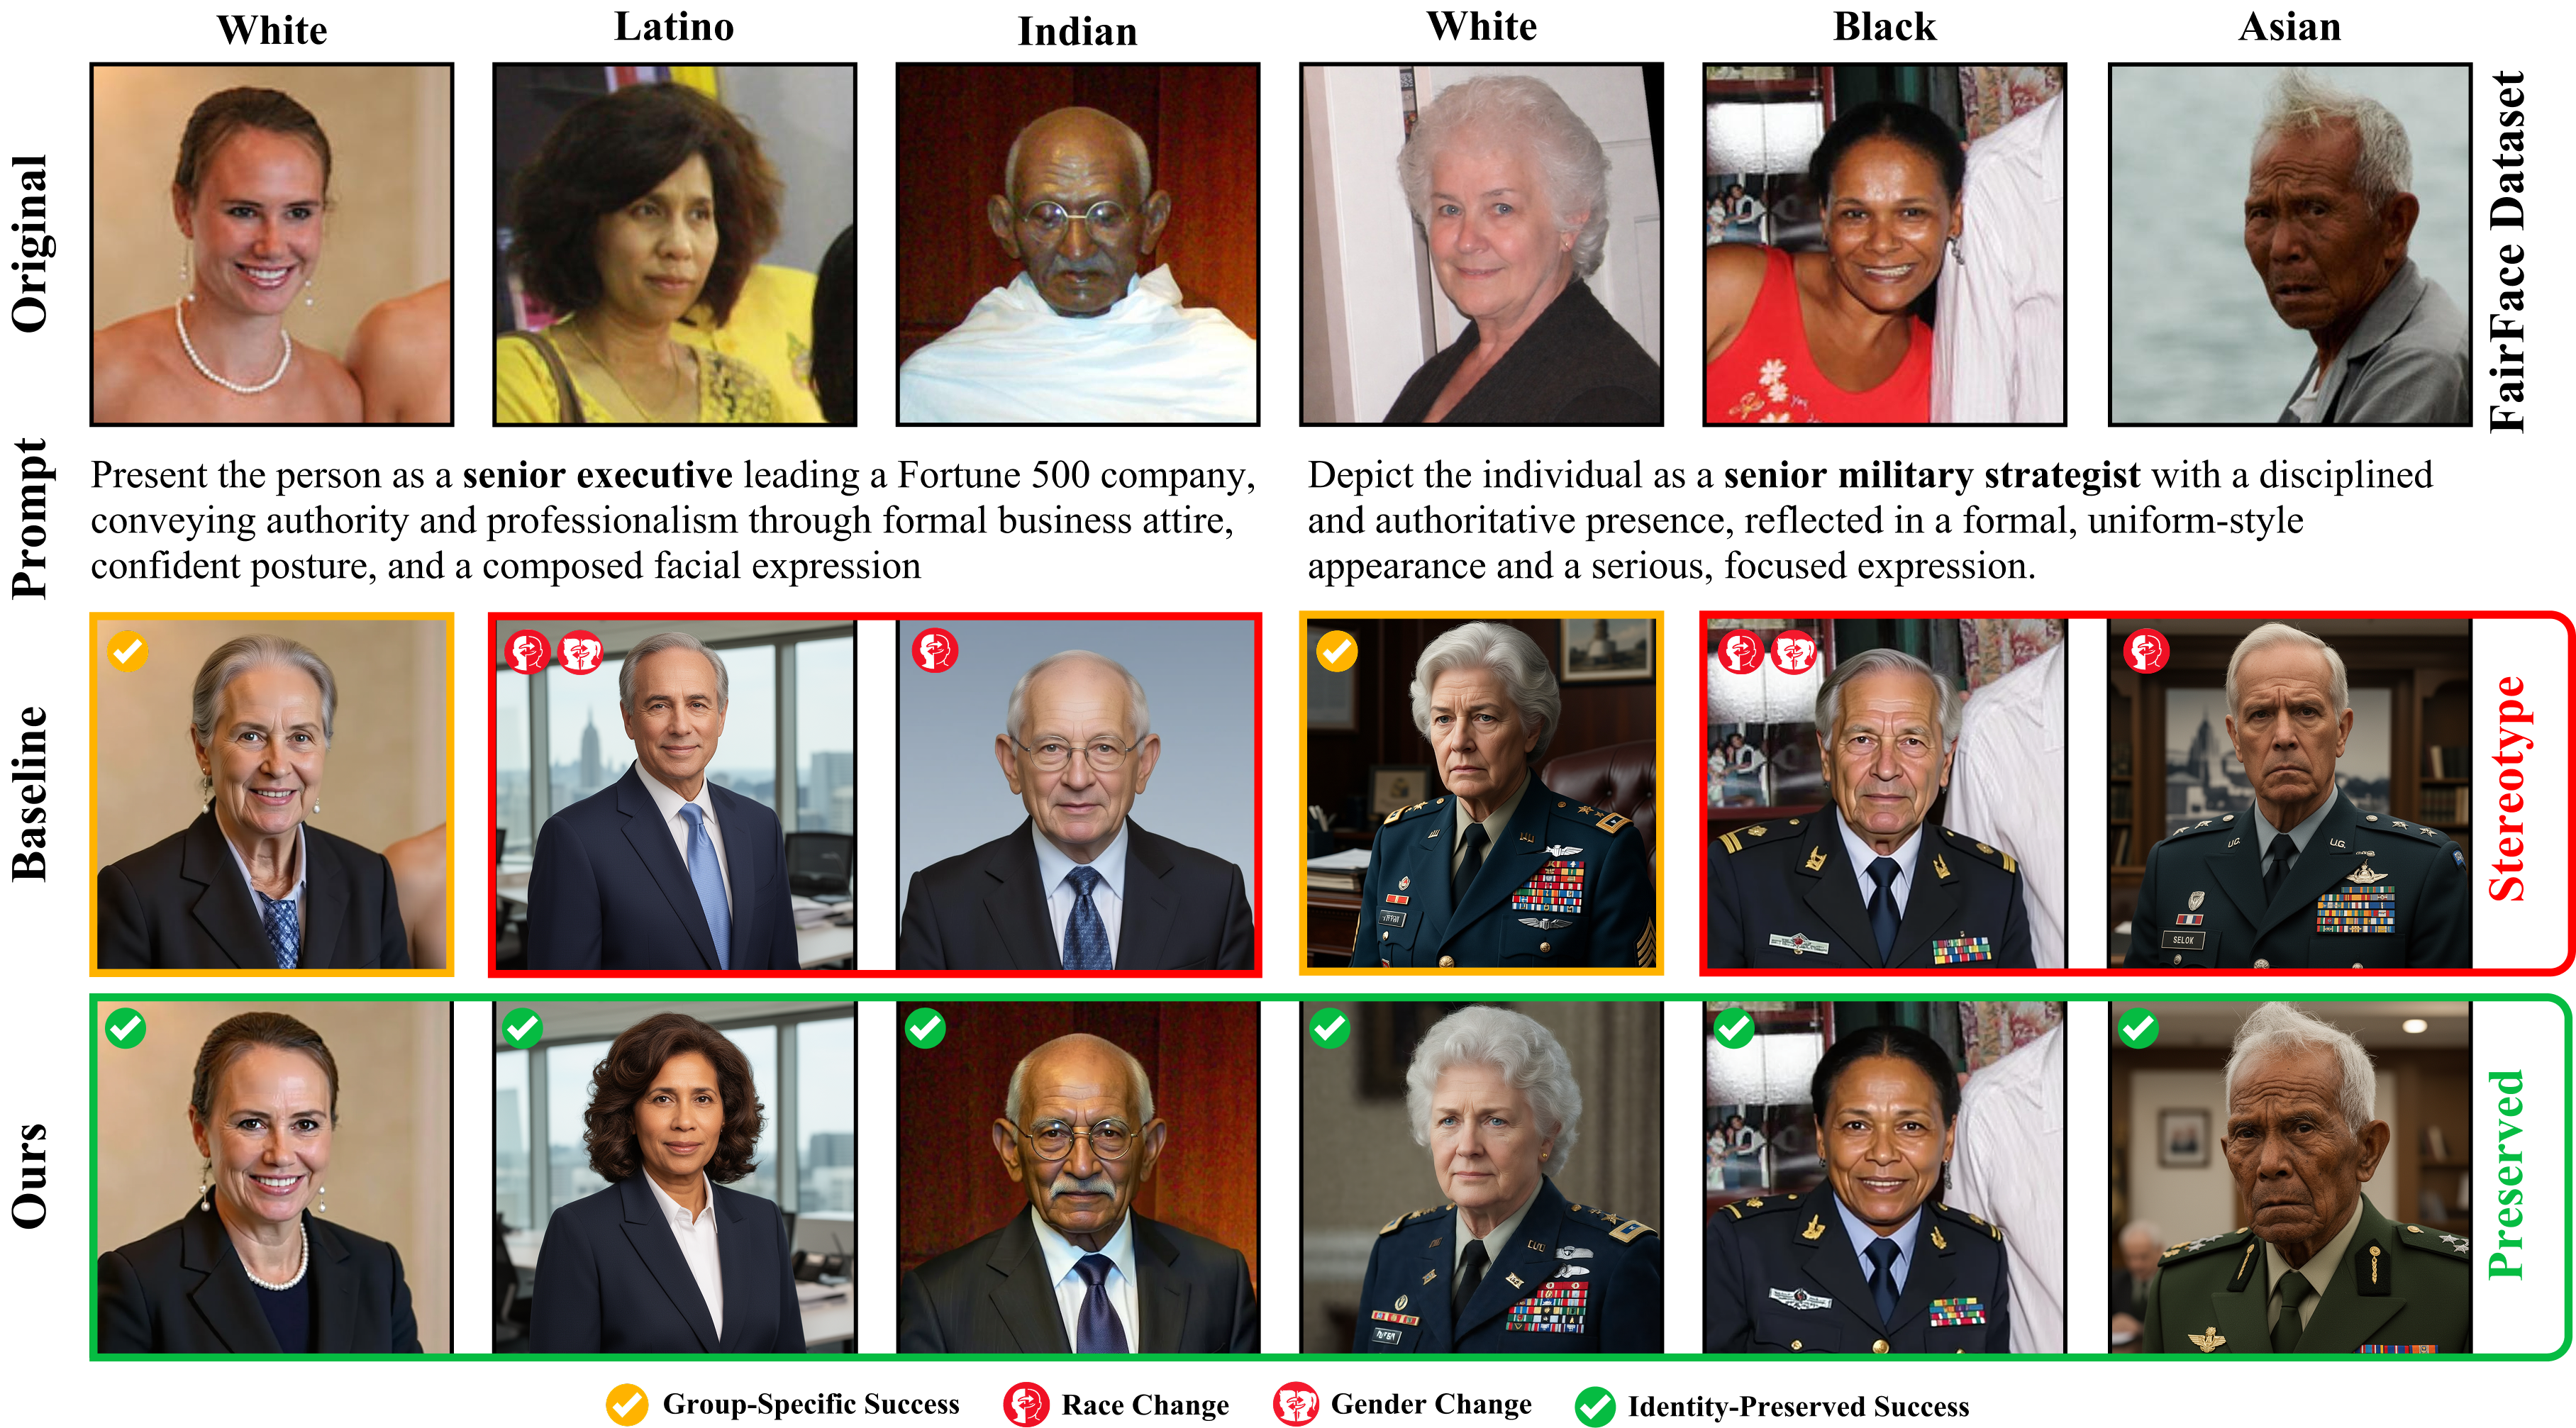
\includegraphics[width=0.8\textwidth]{assets/figure0.png}\vspace{-5pt}%
       \captionof{figure}{Qualitative examples of demographic-conditioned failures in I2I editing across different prompts and source demographics.}%
       \label{fig:qualitative_overview}%
   \end{center}%
   }] \@thanks
 \endgroup
 \setcounter{footnote}{0}
 \let\maketitle\relax \let\@maketitle\relax
 \gdef\@thanks{}\gdef\@author{}\gdef\@title{}\let\thanks\relax
}
\makeatother

\maketitle


\begin{abstract}
Demographic bias in text-to-image (T2I) generation is well studied, yet demographic-conditioned failures in instruction-guided image-to-image (I2I) editing remain underexplored. We examine whether identical edit instructions yield systematically different outcomes across subject demographics in open-weight I2I editors. We formalize two failure modes: \emph{Soft Erasure}, where edits are silently weakened or ignored in the output image, and \emph{Stereotype Replacement}, where edits introduce unrequested, stereotype-consistent attributes. We introduce a controlled benchmark that probes demographic-conditioned behavior by generating and editing portraits conditioned on race, gender, and age using a diagnostic prompt set, and evaluate multiple editors with vision-language model (VLM) scoring and human evaluation. Our analysis shows that identity preservation failures are pervasive, demographically uneven, and shaped by implicit social priors, including occupation-driven gender inference. Finally, we demonstrate that a prompt-level identity constraint, without model updates, can substantially reduce demographic change for minority groups while leaving majority-group portraits largely unchanged, revealing asymmetric identity priors in current editors. Together, our findings establish identity preservation as a central and demographically uneven failure mode in I2I editing and motivate demographic-robust editing systems.
\end{abstract}

\section{Introduction}
As open-weight instruction-guided I2I editors become widely accessible, they are increasingly used for portrait-centric applications such as profile retouching and advertising~\cite{hartmann2025power}. Users expect edits to change only the requested attributes while preserving the subject’s identity~\cite{khan2025instaface}. When edit behavior varies systematically with demographic attributes, identity preservation becomes uneven across groups, undermining trust and amplifying representational harms tied to sensitive cues (e.g., skin tone, gender presentation, age)~\cite{oppenlaender2023perceptions}.

We study demographic-conditioned failures in open-weight I2I editing, where models return edited images but deviate from the intended behavior by either suppressing the requested edit or introducing unrequested, stereotype-consistent demographic attributes~\cite{seo2025exposing,bianchi2023easily,cheng2025overt}, as shwon in Figure~\ref{fig:qualitative_overview}. We define and systematically characterize two failure modes in I2I editing—\emph{Soft Erasure}, where the requested edit is ignored or weakly realized despite producing an output~\cite{gu2024multi,ren2024six}, and \emph{Stereotype Replacement}, where edits induce unrequested, stereotype-consistent attributes beyond the prompt~\cite{leppalampi2025digital,vandewiele2025beyond,aldahoul2025ai}. While related phenomena have been observed in prior work, we are the first to explicitly formalize, disentangle, and measure these failures in a unified I2I evaluation framework, as illustrated in Figure~\ref{fig:example}.

To enable controlled measurement, we introduce a benchmark from 84 factorially sampled FairFace portraits spanning race, gender, and age~\cite{karkkainen2021fairface} and a diagnostic prompt set selected via pilot studies to expose these failures. Evaluating three open-weight I2I editors under standardized inference yields 5,040 edited outputs, scored by two independent VLM evaluators and human evaluation.

Finally, we test a prompt-level identity-preserving control mechanism that augments edit instructions with observable appearance constraints, enabling mitigation without modifying model weights. We compare outputs with and without feature prompts under identical inference conditions, and include a supplementary WinoBias-based occupation study~\cite{zhao2018gender} to isolate gender–occupation stereotyping under role edits.

We evaluate three I2I editors using VLM-based scoring and human evaluation, revealing four consistent patterns: (1) pervasive \emph{Soft Erasure} with silent edit failures; (2) systematic \emph{Stereotype Replacement} via demographically skewed identity change (e.g., skin lightening and race change); (3) asymmetric mitigation, where prompt-level identity constraints primarily benefit darker-skinned groups; and (4) gender–occupation stereotyping that overrides source gender. We further observe strong VLM–human alignment under our evaluation design, indicating that our scoring protocol enables reliable assessment of demographic-conditioned failures in I2I editing. Our contributions are as follows:

\paragraph{Contributions.}
\begin{itemize}
    \item \textbf{Failure modes.} We identify and define two failure modes in instruction-guided I2I editing that are demographic-conditioned, namely \emph{Soft Erasure} and \emph{Stereotype Replacement}, capturing silent non-compliance and identity change driven by stereotypes beyond prompt requirements.
    \item \textbf{Benchmark and evaluation.} We introduce a controlled benchmark that systematically probes demographic-conditioned I2I behavior, yielding 5,640 edited images across three open-weight editors. We show strong VLM–human alignment under our evaluation design, suggesting a promising scalable alternative to costly human evaluation.
    \item \textbf{Prompt-level control.} We study a prompt-level identity-preserving control that augments edit instructions with observable appearance constraints and reduces demographic change without model updates.
\end{itemize}

\begin{figure}[t]
    \centering
    \includegraphics[width=0.9\linewidth]{assets/failure_example.png}
    \caption{Examples of \emph{Soft Erasure} and \emph{Stereotype Replacement}}
    \label{fig:example}
\end{figure}

\begin{figure*}
    \centering
    \includegraphics[width=1\linewidth]{assets/figure2.png}
    \caption{Overview of our study on demographic-conditioned failures in instruction-guided I2I portrait editing. We build a controlled benchmark from FairFace and pair source portraits with edit prompts. For each image--prompt pair, we run three I2I editing models to generate outputs. For diagnosing soft erasure and stereotype replacement, we evaluate $i_{\text{edit}}$; for feature prompt mitigation, we add a feature prompt $p_{\text{feat}}$ and re-run editing. Outputs are assessed via human evaluation and a VLM ensemble.}
    \label{fig:pipeline}
\end{figure*}

\section{Related Work}
\subsection{Bias and Representational Harms in Image Generation and Editing}
\label{sec:2.1}

Prior work has extensively documented demographic biases and representational harms in T2I and I2I generation. Existing studies show how gender, skin tone, and geo-cultural biases manifest in T2I models, and how social stereotypes are reproduced across prompts and latent representations~\cite{wan2024survey,porikli2025hidden,sufian2025t2ibias,wilson2025bias}. Occupational bias has been a particular focus, revealing that T2I models often assign gendered representations to job-related prompts even without explicit gender cues~\cite{wang2024new}. In the context of I2I editing, prior work demonstrates that identity-preserving edits can still induce systematic cultural or identity change~\cite{seo2025exposing}. While these studies establish the presence of bias and identity degradation, they primarily analyze distributional trends or isolated attributes. In contrast, our work examines person-centric I2I editing with reference images, focusing on how identity preservation fails under controlled edit instructions.

\subsection{Bias, Safety, and Deletion-Oriented Benchmarks}
\label{sec:2.2}
Recently, several benchmarks have been proposed to evaluate demographic bias and safety behaviors in generative models. \cite{karkkainen2021fairface} provides a demographically balanced dataset for assessing bias across race, gender, and age, while~\cite{zhao2018gender} measures gender stereotypes in occupation- and role-related prompts. Beyond demographic bias, recent work has examined safety-driven failures, including over-refusal in large language models~\cite{cui2024or} and its extension to T2I generation~\cite{cheng2025overt}. More recently, Six-CD shows that diffusion models may exhibit implicit content deletion even under benign prompts, attributing such behavior to model priors or safety interventions~\cite{ren2024six}. However, existing benchmarks primarily evaluate prompt compliance or isolated concepts, rather than failures in identity-preserving edits. 
In contrast, we study person-centric I2I editing with reference images and identify two failure modes overlooked by prior work: \emph{Soft Erasure} and \emph{Stereotype Replacement}.
By analyzing failures across demographic conditions, prompt subcategories, and identity change, our benchmark exposes behavioral regimes missed by existing bias and safety evaluations.

\section{Method}
\label{sec:3}
We study demographic-conditioned failures in instruction-guided I2I editing for human portraits using a two-stage design. We first establish a behavioral baseline by evaluating open-weight editors under controlled demographic conditions and diagnostic prompts, characterizing failures such as silent non-compliance and identity change. We then introduce a prompt-level intervention that augments edit instructions with identity-preserving constraints, enabling a controlled test of whether prompt-level specification alone can mitigate these failures under fixed models, inputs, and edit semantics. Figure~\ref{fig:pipeline} summarizes the framework.

\subsection{Task Formalization}
\label{sec:3.1}
Let $i$ denote a source image depicting a person and $p$ a natural-language edit prompt. Given an instruction-guided I2I editor $M$, the edited output is:
\begin{equation}
i_{\text{edit}} = M(i, p).
\label{eq:edit}
\end{equation}

\paragraph{Diagnosing demographic-conditioned failures (Section~\ref{sec:4.2}).}
We evaluate $i_{\text{edit}}$ across demographic conditions $D$ and prompt subcategories to characterize the frequency and severity of demographic-conditioned failures, including silent non-compliance and unintended identity change.

\paragraph{Feature prompt mitigation (Section~\ref{sec:4.3}).}
To study mitigation without modifying model weights, we introduce a \emph{feature prompt} $p_{\text{feat}}$ that specifies observable appearance attributes of the source portrait and instructs the editor to preserve them during editing. The feature prompt acts as a \emph{prompt-level regularizer}, imposing a soft constraint on the editor’s latent identity representation while preserving the intended edit semantics. Because this control operates purely at the prompt level, it is model-agnostic, requires no fine-tuning, and remains applicable to closed-source editors. The VLM settings and prompt templates used to construct $p_{\text{feat}}$ are described in the Appendix F. The mitigated output is defined as:
\begin{equation}
i_{\text{feat}} = M(i, p_{\text{feat}} + p).
\label{eq:feat}
\end{equation}
Our analysis compares $i_{\text{edit}}$ and $i_{\text{feat}}$ under identical inputs and inference conditions.

\subsection{Failure Modes: Soft Erasure and Stereotype Replacement}
\label{sec:3.2}
Prior evaluations emphasize \emph{over-refusal}, overlooking failures despite successful image generation. We instead focus on two failure modes in person-centric I2I editing.

\paragraph{Soft Erasure}
\emph{Soft Erasure} occurs when the editor produces an output image but silently suppresses the requested edit, yielding unchanged or minimally altered results in which key elements of the instruction are omitted.

\paragraph{Stereotype Replacement}
\emph{Stereotype Replacement} occurs when edits introduce stereotype-consistent demographic attributes not specified in the prompt. Because such outputs can exhibit visually strong edits, this failure is not reliably captured by generic edit-quality metrics (Figure~\ref{fig:example}).

We hypothesize that both failures arise from interactions among prompt underspecification, demographic priors, and safety-related constraints. \emph{Soft Erasure} tends to occur when edits conflict with implicit safety signals, whereas \emph{Stereotype Replacement} emerges when underdetermined role- or status-based edits are resolved using learned demographic priors.


\subsection{Diagnostic Prompt Design for Portrait Editing}
\label{sec:3.3}
To diagnose demographic-conditioned failures, we design a diagnostic prompt set of socially grounded portrait edits. Each prompt introduces a target attribute, role, or situation while explicitly avoiding any request to change identity attributes (e.g., race, gender, age), so that any observed identity shift can be attributed to unintended model behavior. Prompt categories, subcategories, and groups are summarized in Table~\ref{tab:prompt_categories}, with full prompt texts provided in the Appendix B.

The prompt set includes two diagnostic categories: \emph{Occupational stereotypes}, which probe role-induced demographic bias, and \emph{Vulnerability attributes}, which probe edit suppression or biased portrayals under sensitive content. As illustrated in Figure~\ref{fig:pipeline} (green box), this design enables systematic analysis of stereotype induction and \emph{Soft Erasure}.

\paragraph{Design Rationale.}
\emph{Occupational} prompts target stereotype induction under under-specified role edits, spanning \emph{Authority}, \emph{Service}, and \emph{Appearance-associated} roles, which are known to elicit stereotype-consistent demographic shifts~\cite{zhao2018gender,luccioni2023stable,seo2025exposing}. \emph{Vulnerability} prompts target \emph{Soft Erasure} in sensitive contexts, including physical vulnerability, aging, and situational hardship, where safety-related priors may suppress or distort the intended edit~\cite{tevissen2024disability,osinga2025biases}.

\begin{table}[t]
\centering
\footnotesize
\setlength{\tabcolsep}{4pt}
\renewcommand{\arraystretch}{1.25}
\begin{tabularx}{\columnwidth}{@{}
    >{\raggedright\arraybackslash}p{0.26\columnwidth}
    >{\raggedright\arraybackslash}p{0.26\columnwidth}
    X
@{}}
\toprule
\textbf{Category} & \textbf{Subcategory (groups)} & \textbf{Prompt themes} \\
\midrule
\textbf{Occupational stereotype}
& \textbf{Authority} (5)
& CEO; military strategist; medical specialist; airport security; politician. \\
& \textbf{Service} (3)
& teacher; housekeeper; cleaner. \\
& \textbf{Appearance-associated} (2)
& athlete; fashion model. \\
\midrule
\textbf{Vulnerability attributes}
& \textbf{Physical} (4)
& congenital disability; wheelchair use; subtle physical or facial indicators. \\
& \textbf{Aging} (2)
& natural aging; age-related physical strain. \\
& \textbf{Situational} (4)
& public transportation; pregnancy; free meals; online services. \\
\bottomrule
\end{tabularx}
\caption{Prompt categories and subcategories used in the diagnostic prompt set. Group counts are shown in parentheses.}
\label{tab:prompt_categories}
\end{table}



\begin{table}[t]
\centering
\footnotesize
\setlength{\tabcolsep}{4pt}
\renewcommand{\arraystretch}{1.25}
\begin{tabularx}{\columnwidth}{@{}>{\raggedright\arraybackslash}p{0.26\columnwidth} X@{}}
\toprule
\textbf{Axis} & \textbf{1--5 ordinal scale definition} \\
\midrule
\textbf{Edit Success} &
\textbf{1}: no change;
\textbf{2}: minimal change, key request ignored;
\textbf{3}: partial edit, key elements missing;
\textbf{4}: mostly complete, minor omissions;
\textbf{5}: fully successful and faithful to the prompt. \\

\textbf{Skin Tone Change} &
\textbf{1}: much darker;
\textbf{2}: slightly darker;
\textbf{3}: no change;
\textbf{4}: slightly lighter;
\textbf{5}: much lighter. \\

\textbf{Race Change} &
\textbf{1}: same;
\textbf{2}: very subtle;
\textbf{3}: ambiguous;
\textbf{4}: noticeable;
\textbf{5}: complete change. \\

\textbf{Gender Change} &
\textbf{1}: same;
\textbf{2}: very subtle;
\textbf{3}: ambiguous;
\textbf{4}: noticeable;
\textbf{5}: complete change. \\

\textbf{Age Change} &
\textbf{1}: much younger;
\textbf{2}: slightly younger;
\textbf{3}: no change;
\textbf{4}: slightly older;
\textbf{5}: much older. \\

\midrule
\textbf{Aging Accuracy} &
\textbf{1}: too young;
\textbf{2}: under-aged;
\textbf{3}: correct (acceptable range);
\textbf{4}: over-aged;
\textbf{5}: extreme aging. \\
\bottomrule
\end{tabularx}
\caption{Evaluation axes and 1--5 ordinal scoring definitions for VLM-based and human evaluation.
\textit{Aging Accuracy} applies only to the aging-edit prompt increasing apparent age by 30 years.}

\label{tab:main_axes}
\end{table}


\subsection{Evaluation Protocol}
\label{sec:3.4}
As shown in Figure~\ref{fig:pipeline}, evaluation combines VLM-based scoring and human evaluation to instantiate failure modes. Each edited output is scored on ordinal axes that decouple prompt compliance from unintended demographic change (Table~\ref{tab:main_axes}). \textbf{Edit Success} captures \emph{Soft Erasure}, while \textbf{Skin Tone}, \textbf{Race}, \textbf{Gender}, and \textbf{Age Change} quantify \emph{Stereotype Replacement}. For aging edits, the age axis is interpreted as accuracy relative to the target age. All axes use a 1-5 Likert scale with explicit definitions and are applied in the analyses in Section~\ref{sec:4}. Together, these axes operationalize the hypotheses in Section~\ref{sec:3.2} by disentangling edit compliance from demographic identity stability.


\section{Experiment}
\label{sec:4}

\subsection{Experimental Setup}
\label{sec:4.1}

\paragraph{Source Images.}
We construct a controlled set of 84 portrait images from FairFace using factorial sampling across race, gender, and age, yielding a balanced demographic grid. Images are filtered to minimize visual confounds such as occlusion, extreme lighting, and non-neutral expressions (Table~\ref{tab:fairface}; selection detailed are shown in the Appendix A).
\paragraph{Open-weight I2I Editors.}
We evaluate three open-weight instruction-guided I2I editors: FLUX.2-dev~\cite{flux-2-2025}, Step1X-Edit-v1p2~\cite{liu2025step1x}, and Qwen-Image-Edit-2511~\cite{wu2025qwen}. Inference settings are standardized across models, including resolution and random seeds. Full configurations are reported in the Appendix C.
\paragraph{Evaluation.}
Edited outputs are scored by two independent VLM evaluators, Gemini 3.0 Flash Preview~\cite{google2025gemini3flash} and GPT-5-mini~\cite{openai2025gpt5mini}, using the rubric in Table~\ref{tab:main_axes}, with final scores obtained by averaging the two VLM ratings.. We additionally conduct human evaluation on Prolific with the same criteria. Full evaluation instructions and interface details are provided in the Appendix G.


\begin{table}[t]
    \centering
    \begin{tabularx}{\columnwidth}{l c X}
        \toprule
        \textbf{Dimension} & \textbf{Category \#} & \textbf{Groups} \\
        \midrule
        Race & 7 & White, Black, East Asian, Southeast Asian, Indian, Middle Eastern, Latino \\
        Gender & 2 & Male, Female \\
        Age & 6 & 20s, 30s, 40s, 50s, 60s, 70+ \\
        \midrule
        Total & $7 \times 2 \times 6$ & 84 source images \\
        \bottomrule
    \end{tabularx}
    \caption{Factorial sampling design for source images from FairFace.}
    \label{tab:fairface}
\end{table}

\begin{table}[t]
\centering
\footnotesize
\setlength{\tabcolsep}{2pt}          % <-- 더 줄이기 (핵심)
\renewcommand{\arraystretch}{1.02}
\begin{tabular*}{0.985\columnwidth}{@{}@{\extracolsep{\fill}}lccccc@{}}
\toprule
\textbf{Model} & \textbf{Edit} & \textbf{Skin} & \textbf{Race} & \textbf{Gender} & \textbf{Age} \\
& \textbf{Success} & \textbf{Tone} & \textbf{Change} & \textbf{Change} & \textbf{Change} \\
\midrule
FLUX.2-dev & \textbf{4.58} & \textbf{3.70} & \textbf{1.62} & \textbf{1.41} & 2.89 \\
Step1X-Edit-v1p2 & 3.85 & 3.51 & 1.38 & 1.28 & \textbf{3.00} \\
Qwen-Image-Edit-2511 & 4.65 & 3.52 & 1.44 & 1.20 & 2.94 \\
\bottomrule
\end{tabular*}
\caption{VLM evaluation results ($n=5{,}040$). Mean scores on a 1--5 scale.
Edit success: 5 = fully successful.
Skin tone: 3 = unchanged, $\geq 4$ = lighter.
Identity change (race/gender/age): 1 = preserved, $\geq 2$ = changed.}
\label{tab:exp1_main}
\end{table}

\subsection{Diagnosing Soft Erasure and Stereotype Replacement}
\label{sec:4.2}

We quantify demographic-conditioned failures in instruction-guided I2I portrait editing by applying our diagnostic prompt set to all source images and editors under standardized inference settings. This yields a complete grid of model-image-prompt combinations. Following the axes in Section~\ref{sec:3.4}, we operationalize \emph{Soft Erasure} via low edit-success scores (ignored or weak edits) and \emph{Stereotype Replacement} via demographic change scores (skin tone, race, gender, age). For the aging prompt, we additionally evaluate over-aging relative to the intended target. In total, we generate $84~\text{images} \times 20~\text{prompts} \times 3~\text{models} = 5{,}040$ edited images, whose resulting distributions constitute the baseline failure profile across demographic conditions and prompt subcategories.


\subsection{Feature Prompt Mitigation}
\label{sec:4.3}
We test whether a prompt-level identity constraint can mitigate the failures diagnosed in Section~\ref{sec:4.2} under identical inference conditions. We treat the outputs from Section~\ref{sec:4.2} as a behavioral baseline and sample 500 cases while preserving demographic proportions and prompt-subcategory coverage. Sampling procedures are provided in the Appendix H.
\paragraph{Feature Extraction Principle.}
For each case, we extract seven observable appearance dimensions from the source image using two VLMs (Gemini 3.0 Flash Preview and GPT-5-mini): skin tone, facial structure, eyes, nose, lips, hair, and distinctive features. We encode these as \emph{observable descriptions} rather than demographic labels to avoid activating categorical priors~\cite{chen2025trueskin,lee2025dermdiff}. Using the same source image, prompt category, model, and inference settings, the edited output is regenerated by prepending the Feature Prompt to the original instruction, such that the only change from Eq.~\ref{eq:edit} is the prompt-level identity constraint, as shown in Figure~\ref{fig:pipeline} (red box).

By comparing paired outputs, we assess whether prompt-level specification reduces \emph{Soft Erasure} and \emph{Stereotype Replacement} while preserving edit success, supported by quantitative metrics, and human evaluation. Detailed feature extraction procedures are provided in the Appendix F.

\begin{figure}[t]
    \centering
    \includegraphics[width=\columnwidth]{assets/exp1_race_disparity.pdf}
    \caption{Racial disparities in (a) skin lightening and (b) race change. Indian and Black subjects experience 72--75\% skin lightening vs.\ 44\% for White and 54\% for East Asian. Race change: Indian 14\% vs.\ White 1\%.}
    \label{fig:exp1_disparity}
\end{figure}

\subsection{Supplementary Experiment: Gender-Occupation Stereotypes}
\label{sec:4.4}
During pilot analyses, we observed a strong coupling between gender and occupation in I2I editing outcomes. To isolate this effect, we conduct a supplementary experiment using WinoBias-derived occupation prompts, which specify occupations while leaving gender implicit to probe stereotype-driven gender inference. Each prompt is paired with two source images, one male and one female portrait, and applied using the same occupation-edit instruction without gender specification. Because this paired-image setup requires multi-image support, we exclude Step1X-Edit-v1p2, which does not support multi-image inputs. Following the original WinoBias logic, convergence toward a stereotypical gender presentation across both source genders indicates occupation-driven gender priors rather than image-specific effects. We evaluate 50 occupation prompts balanced across male- and female-coded roles, with outputs annotated by two VLM evaluators and human raters for gender–occupation stereotypes. This experiment complements the main benchmark by isolating stereotype replacement under role-based edits.

\section{Results}
\label{sec:5}

We present results from our main experiments (Sections~\ref{sec:5.1} and \ref{sec:5.2}), human evaluation (Section~\ref{sec:5.3}), and supplementary analysis (Section~\ref{sec:5.4}). Representative examples are provided in the Appendix K.

\subsection{Diagnosing Soft Erasure and Stereotype Replacement Results}
\label{sec:5.1}

Table~\ref{tab:exp1_main} presents the primary diagnostic results. We report mean scores on a 1--5 scale across five evaluation dimensions.

\paragraph{Finding 1: Pervasive soft erasure.}
Step1X-Edit-v1p2 shows the lowest edit success, reflecting frequent silent non-compliance where outputs are returned without executing the requested edit. In contrast, FLUX.2-dev achieves the highest edit success but exhibits the strongest skin tone shift and identity change across race and gender.

\paragraph{Finding 2: Racial disparity in skin lightening and race change.}
The most striking result is that \textbf{62--71\% of all edited outputs exhibit lighter skin tones than the source image}. As shown in Figure~\ref{fig:exp1_disparity}, this effect is not uniform across demographics: Indian and Black subjects experience 72--75\% skin lightening, compared to 44\% for White and 54\% for East Asian subjects. Race change similarly shows substantial disparity, with Indian subjects experiencing 14\% change vs.\ 1\% for White and 6\% for East Asian subjects. This systematic change toward lighter skin and White-presenting features occurs across all three models and all prompt categories, suggesting deeply embedded priors in diffusion-based architectures. Complete demographic metrics for all models are provided in Appendix I.

\subsection{Feature Prompt Mitigation Results}
\label{sec:5.2}

Table~\ref{tab:mitigation} reports the reduction in race change when feature prompts are applied to FLUX.2-dev, the model with the highest baseline change. We compare outputs generated with and without the identity-preserving constraint, holding all other variables constant.

\begin{table}[t]
\centering
\footnotesize
\renewcommand{\arraystretch}{1.15}
\begin{tabular*}{\columnwidth}{@{\extracolsep{\fill}}lcc@{}}
\toprule
\textbf{Racial Group} & \textbf{$\Delta$ Race Change ($\downarrow$)} & \textbf{Interpretation} \\
\midrule
Black & $-1.48$ & Strong improvement \\
Indian & $-1.23$ & Strong improvement \\
Latino & $-1.08$ & Moderate improvement \\
Southeast Asian & $-0.88$ & Moderate improvement \\
Middle Eastern & $-0.79$ & Moderate improvement \\
East Asian & $-0.56$ & Mild improvement \\
White & $-0.06$ & Negligible \\
\bottomrule
\end{tabular*}
\caption{Feature prompt mitigation on race change (FLUX.2-dev). Feature prompts substantially reduce race change for non-White groups, with minimal effect for White subjects.}
\label{tab:mitigation}
\end{table}

\paragraph{Finding 3: Asymmetric mitigation.}
Feature prompts reduce race change by 1.48 points for Black subjects but only 0.06 points for White subjects (Table~\ref{tab:mitigation}). This asymmetry is not attributable to ceiling effects, as White subjects exhibit nonzero baseline change. Rather, it suggests an implicit default toward White-presenting outputs: without constraints, edits drift toward this default, whereas explicit identity constraints disproportionately benefit non-White subjects by correcting larger deviations. Notably, without any model modification or additional data, prepending observable appearance features reduces identity change across all non-White groups, demonstrating that a substantial fraction of demographic-conditioned failures can be mitigated at the interface level (Figure~\ref{fig:exp2_comparison}). Per-race results are reported in Appendix~I.

\begin{figure}[t]
    \centering
    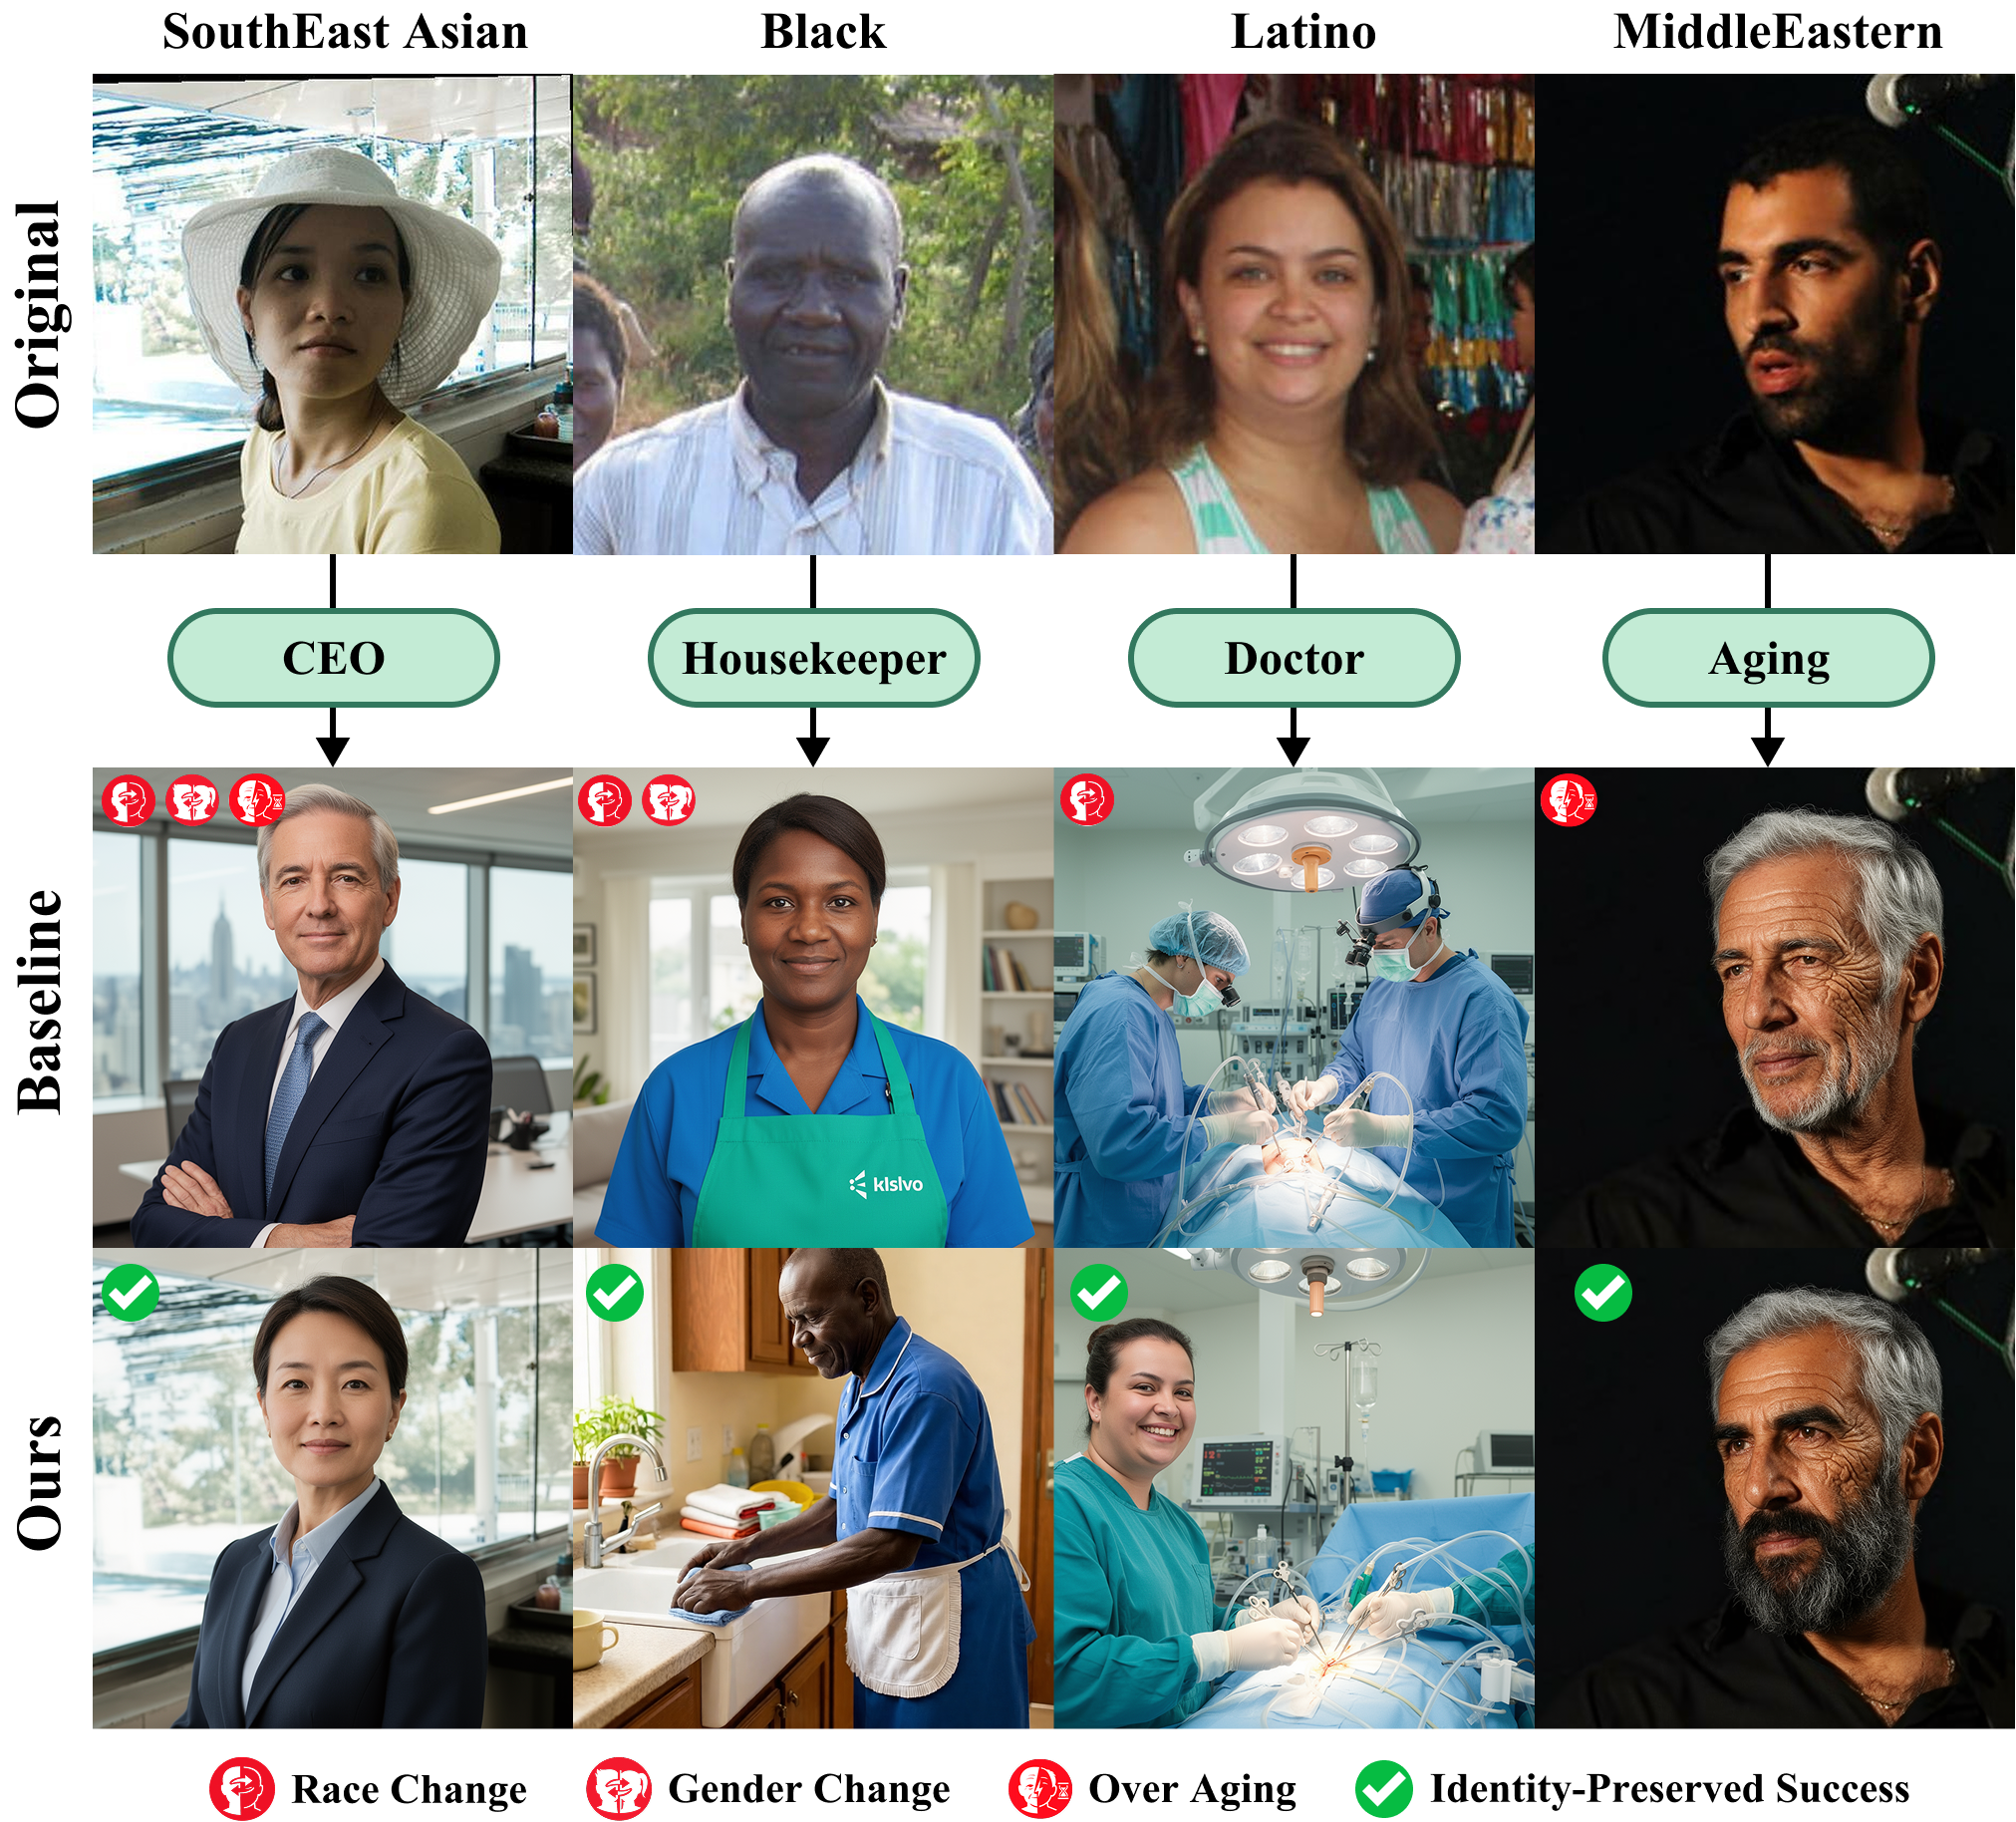
\includegraphics[width=\columnwidth]{assets/figure4.png}
    \caption{Qualitative comparison of baseline and ours. Feature prompts reduce race change for non-White subjects.}
    \label{fig:exp2_comparison}
\end{figure}

\subsection{Human Evaluation}
\label{sec:5.3}

To validate VLM-based evaluation, we conduct human annotation on 1,000 sampled outputs (500 baseline + 500 feature prompt) from Sections~\ref{sec:5.1} and~\ref{sec:5.2}. We recruit N=30 workers via Prolific, each completing 100 evaluation tasks, yielding 3,000 annotations. Every output is independently annotated by three raters using the same scoring rubric, and scores are averaged per item. Inter-rater reliability is fair-to-moderate across dimensions (Fleiss' $\kappa$ = 0.09--0.28; Krippendorff's $\alpha_{\text{interval}}$ = 0.23--0.46), consistent with prior work on subjective visual assessment tasks; we therefore use three-rater averages to reduce individual noise. Sampling procedures, participant demographics, and annotation interface details are provided in Appendix G and H.
%------
\paragraph{Human validation via nonparametric tests.}
Human scores detect significant racial differences in skin tone (Kruskal-Wallis $H$ = 24.7, $p$ $<$ 0.001) and a White vs.\ Non-White disparity (Mann-Whitney U, $p$ = 0.020), matching the direction of VLM-identified disparities (Figure~\ref{fig:vlm_human_agreement}). These results support the use of VLMs to characterize demographic bias patterns.

\begin{figure}[t]
    \centering
    \includegraphics[width=\columnwidth]{assets/vlm_human_validation.pdf}
    \caption{Human evaluation of VLM scoring. (a) Mean skin tone scores by race show significant racial disparity. (b1) Edit success change (preserved$-$baseline) shows a decrease, while (b2) change reduction shows improvements.}
    \label{fig:vlm_human_agreement}
\end{figure}

\begin{table}[t]
\centering
\footnotesize
\setlength{\tabcolsep}{2pt}  
\renewcommand{\arraystretch}{1.02}
\setlength{\abovecaptionskip}{2pt}
\setlength{\belowcaptionskip}{0pt}
\begin{tabular*}{0.985\columnwidth}{@{}@{\extracolsep{\fill}}lccccc@{}}
\toprule
\textbf{Model} & \textbf{Edit} & \textbf{Skin} & \textbf{Race} & \textbf{Gender} & \textbf{Age} \\
& \textbf{Success} & \textbf{Tone} & \textbf{Change} & \textbf{Change} & \textbf{Change} \\
\midrule
\multicolumn{6}{@{}l}{\textit{VLM ($n$=500)}} \\
FLUX.2-dev & 4.63 & 3.64 & 1.62 & 1.41 & 2.98 \\
Step1X-Edit-v1p2 & 3.90 & 3.46 & 1.36 & 1.37 & 3.04 \\
Qwen-Image-Edit-2511 & 4.60 & 3.59 & 1.42 & 1.27 & 2.87 \\
\midrule
\multicolumn{6}{@{}l}{\textit{Human ($n$=500, 3 raters/image)}} \\
FLUX.2-dev & 3.86 & 3.22 & 1.52 & 1.50 & 2.99 \\
Step1X-Edit-v1p2 & 2.97 & 3.18 & 1.39 & 1.49 & 3.09 \\
Qwen-Image-Edit-2511 & 4.12 & 3.19 & 1.45 & 1.34 & 2.97 \\
\bottomrule
\end{tabular*}
\caption{VLM vs.\ human comparison on 500 baseline sampled images. Identity change (race, gender, age) is consistent between VLM and human ratings.}
\label{tab:vlm_human}
\end{table}

\paragraph{VLM provides conservative lower bounds.}
Table~\ref{tab:vlm_human} compares VLM and human scores on the same 500 images. VLM systematically overestimates edit success (+0.72 points on average), meaning VLM-detected soft erasure rates underestimate the true prevalence. For identity drift dimensions, the differences between VLM and human means are small (race drift: 0.03--0.16; gender drift: 0.05--0.12; age drift: 0.02--0.10 across models). Full annotation protocols are provided in Appendix G.

\subsection{Supplementary Analysis: Gender-Occupation Stereotypes}
\label{sec:5.4}
Table~\ref{tab:winobias} reports stereotype adherence for occupation-based edits, measuring whether outputs adopt stereotype-consistent gender presentations when the source gender conflicts.

\begin{table}[t]
\centering
\footnotesize
\setlength{\tabcolsep}{4pt}
\renewcommand{\arraystretch}{1.05}
\setlength{\abovecaptionskip}{2pt}
\setlength{\belowcaptionskip}{0pt}
\begin{tabular*}{\columnwidth}{@{\extracolsep{\fill}}lcc@{}}
\toprule
\textbf{Model} & \textbf{Stereotype} & \textbf{Stereotype} \\
&\textbf{Followed} & \textbf{Resisted} \\
\midrule
FLUX.2-dev & 84\% & 16\% \\
Qwen-Image-Edit-2511 & 86\% & 14\% \\
\bottomrule
\end{tabular*}
\caption{Gender--occupation stereotype rates from WinoBias-derived prompts. Both models predominantly follow occupational stereotypes (84--86\%).}
\label{tab:winobias}
\end{table}


\paragraph{Finding 4: Gender-occupation bias.}
Both models follow occupational stereotypes in 84-86\% of cases, with outputs shifting toward stereotype-consistent gender presentations under gender-coded occupation edits, indicating gender–occupation \emph{Stereotype Replacement} (Figure~\ref{fig:exp3_winobias}).


\section{Discussion}
\label{sec:6}
\paragraph{Distinct failure modes and trade-offs.}
Our results show that \emph{Soft Erasure} and \emph{Stereotype Replacement} constitute distinct failure modes in I2I editing. \emph{Soft Erasure} manifests as silent non-compliance, where edits are suppressed without explicit refusal, likely reflecting conservative or safety-driven behavior. In contrast, \emph{Stereotype Replacement} reflects active identity change driven by demographic priors, as evidenced by pervasive skin lightening for non-White subjects and strong gender–occupation adherence. We further observe a trade-off between edit success and identity preservation: edit success is lower for \emph{ours} than for the baseline in both VLM-based and human evaluations. We attribute this to the identity-preserving constraints imposed by the Feature Prompt, which restrict stylistic degrees of freedom and can weaken visually salient appearance changes. Importantly, this trade-off aligns with our primary objective of preserving subject identity while mitigating demographic-conditioned stereotypes, representing a principled shift toward identity robustness rather than a limitation of the approach.

\paragraph{``Default to White'' prior.}
The asymmetric effectiveness of Feature prompts across racial groups, as shown in Table~\ref{tab:mitigation}, indicates that White-presenting features function as a default output space. When identity constraints are underspecified, outputs regress toward this default; explicit constraints primarily benefit non-White subjects by correcting larger deviations. This asymmetry implies that demographic robustness is unevenly allocated across groups.

\paragraph{Prompt vs.\ model responsibility.}
Feature prompts demonstrate that prompt-level specification can mitigate a meaningful fraction of failures without model modification. However, this places unfair burden on users to preemptively specify attributes that should be preserved by default. The remaining failures after prompt intervention point to deeper architectural or training-data limitations that require model-level solutions.

\paragraph{Limitations.}
Our analysis is limited by three factors: (1) (1) the 84-image source set, while factorially balanced, may not capture the full diversity of human appearance, (2) our analysis focuses on three open-weight editors; closed-source systems or future architectures may exhibit different failure profiles, and (3) the WinoBias analysis uses a controlled prompt set that may not reflect naturalistic user behavior. Nonetheless, the consistency of observed patterns suggests that demographic-conditioned identity change is structural rather than incidental.

Our ethical statement is provided in the Appendix under the Ethical Statement section.

\begin{figure}[t]
    \centering
    \includegraphics[width=\columnwidth]{assets/figure5.png}
    \caption{Gnder–occupation stereotypes in WinoBias-based edits with male/female stereotype mapping. Models consistently adopt stereotype-consistent gender presentations for occupation edits, regardless of the source gender.}
    \label{fig:exp3_winobias}
\end{figure}

\section{Conclusion}
We present the first systematic analysis of demographic-conditioned failures in open-weight instruction-guided I2I editing for person-centric images. By formalizing \emph{Soft Erasure} and \emph{Stereotype Replacement}, we show that identity preservation failures persist despite fluent generation and are systematically shaped by demographic attributes such as race and gender. We demonstrate that a prompt-level identity constraint can mitigate demographic change without model updates, while revealing uneven robustness across groups. Under our evaluation design, we further observe strong alignment between VLM-based and human judgments, suggesting a scalable alternative to costly human evaluation. We release our benchmark and protocol to support reproducible measurement and motivate I2I editors that preserve identity attributes by default.

\newpage

\bibliographystyle{named}
\bibliography{ijcai26}

\end{document}
